% Options for packages loaded elsewhere
\PassOptionsToPackage{unicode}{hyperref}
\PassOptionsToPackage{hyphens}{url}
%
\documentclass[
]{book}
\usepackage{amsmath,amssymb}
\usepackage{iftex}
\ifPDFTeX
  \usepackage[T1]{fontenc}
  \usepackage[utf8]{inputenc}
  \usepackage{textcomp} % provide euro and other symbols
\else % if luatex or xetex
  \usepackage{unicode-math} % this also loads fontspec
  \defaultfontfeatures{Scale=MatchLowercase}
  \defaultfontfeatures[\rmfamily]{Ligatures=TeX,Scale=1}
\fi
\usepackage{lmodern}
\ifPDFTeX\else
  % xetex/luatex font selection
\fi
% Use upquote if available, for straight quotes in verbatim environments
\IfFileExists{upquote.sty}{\usepackage{upquote}}{}
\IfFileExists{microtype.sty}{% use microtype if available
  \usepackage[]{microtype}
  \UseMicrotypeSet[protrusion]{basicmath} % disable protrusion for tt fonts
}{}
\makeatletter
\@ifundefined{KOMAClassName}{% if non-KOMA class
  \IfFileExists{parskip.sty}{%
    \usepackage{parskip}
  }{% else
    \setlength{\parindent}{0pt}
    \setlength{\parskip}{6pt plus 2pt minus 1pt}}
}{% if KOMA class
  \KOMAoptions{parskip=half}}
\makeatother
\usepackage{xcolor}
\usepackage{color}
\usepackage{fancyvrb}
\newcommand{\VerbBar}{|}
\newcommand{\VERB}{\Verb[commandchars=\\\{\}]}
\DefineVerbatimEnvironment{Highlighting}{Verbatim}{commandchars=\\\{\}}
% Add ',fontsize=\small' for more characters per line
\usepackage{framed}
\definecolor{shadecolor}{RGB}{248,248,248}
\newenvironment{Shaded}{\begin{snugshade}}{\end{snugshade}}
\newcommand{\AlertTok}[1]{\textcolor[rgb]{0.94,0.16,0.16}{#1}}
\newcommand{\AnnotationTok}[1]{\textcolor[rgb]{0.56,0.35,0.01}{\textbf{\textit{#1}}}}
\newcommand{\AttributeTok}[1]{\textcolor[rgb]{0.13,0.29,0.53}{#1}}
\newcommand{\BaseNTok}[1]{\textcolor[rgb]{0.00,0.00,0.81}{#1}}
\newcommand{\BuiltInTok}[1]{#1}
\newcommand{\CharTok}[1]{\textcolor[rgb]{0.31,0.60,0.02}{#1}}
\newcommand{\CommentTok}[1]{\textcolor[rgb]{0.56,0.35,0.01}{\textit{#1}}}
\newcommand{\CommentVarTok}[1]{\textcolor[rgb]{0.56,0.35,0.01}{\textbf{\textit{#1}}}}
\newcommand{\ConstantTok}[1]{\textcolor[rgb]{0.56,0.35,0.01}{#1}}
\newcommand{\ControlFlowTok}[1]{\textcolor[rgb]{0.13,0.29,0.53}{\textbf{#1}}}
\newcommand{\DataTypeTok}[1]{\textcolor[rgb]{0.13,0.29,0.53}{#1}}
\newcommand{\DecValTok}[1]{\textcolor[rgb]{0.00,0.00,0.81}{#1}}
\newcommand{\DocumentationTok}[1]{\textcolor[rgb]{0.56,0.35,0.01}{\textbf{\textit{#1}}}}
\newcommand{\ErrorTok}[1]{\textcolor[rgb]{0.64,0.00,0.00}{\textbf{#1}}}
\newcommand{\ExtensionTok}[1]{#1}
\newcommand{\FloatTok}[1]{\textcolor[rgb]{0.00,0.00,0.81}{#1}}
\newcommand{\FunctionTok}[1]{\textcolor[rgb]{0.13,0.29,0.53}{\textbf{#1}}}
\newcommand{\ImportTok}[1]{#1}
\newcommand{\InformationTok}[1]{\textcolor[rgb]{0.56,0.35,0.01}{\textbf{\textit{#1}}}}
\newcommand{\KeywordTok}[1]{\textcolor[rgb]{0.13,0.29,0.53}{\textbf{#1}}}
\newcommand{\NormalTok}[1]{#1}
\newcommand{\OperatorTok}[1]{\textcolor[rgb]{0.81,0.36,0.00}{\textbf{#1}}}
\newcommand{\OtherTok}[1]{\textcolor[rgb]{0.56,0.35,0.01}{#1}}
\newcommand{\PreprocessorTok}[1]{\textcolor[rgb]{0.56,0.35,0.01}{\textit{#1}}}
\newcommand{\RegionMarkerTok}[1]{#1}
\newcommand{\SpecialCharTok}[1]{\textcolor[rgb]{0.81,0.36,0.00}{\textbf{#1}}}
\newcommand{\SpecialStringTok}[1]{\textcolor[rgb]{0.31,0.60,0.02}{#1}}
\newcommand{\StringTok}[1]{\textcolor[rgb]{0.31,0.60,0.02}{#1}}
\newcommand{\VariableTok}[1]{\textcolor[rgb]{0.00,0.00,0.00}{#1}}
\newcommand{\VerbatimStringTok}[1]{\textcolor[rgb]{0.31,0.60,0.02}{#1}}
\newcommand{\WarningTok}[1]{\textcolor[rgb]{0.56,0.35,0.01}{\textbf{\textit{#1}}}}
\usepackage{longtable,booktabs,array}
\usepackage{calc} % for calculating minipage widths
% Correct order of tables after \paragraph or \subparagraph
\usepackage{etoolbox}
\makeatletter
\patchcmd\longtable{\par}{\if@noskipsec\mbox{}\fi\par}{}{}
\makeatother
% Allow footnotes in longtable head/foot
\IfFileExists{footnotehyper.sty}{\usepackage{footnotehyper}}{\usepackage{footnote}}
\makesavenoteenv{longtable}
\usepackage{graphicx}
\makeatletter
\def\maxwidth{\ifdim\Gin@nat@width>\linewidth\linewidth\else\Gin@nat@width\fi}
\def\maxheight{\ifdim\Gin@nat@height>\textheight\textheight\else\Gin@nat@height\fi}
\makeatother
% Scale images if necessary, so that they will not overflow the page
% margins by default, and it is still possible to overwrite the defaults
% using explicit options in \includegraphics[width, height, ...]{}
\setkeys{Gin}{width=\maxwidth,height=\maxheight,keepaspectratio}
% Set default figure placement to htbp
\makeatletter
\def\fps@figure{htbp}
\makeatother
\setlength{\emergencystretch}{3em} % prevent overfull lines
\providecommand{\tightlist}{%
  \setlength{\itemsep}{0pt}\setlength{\parskip}{0pt}}
\setcounter{secnumdepth}{5}
\ifLuaTeX
\usepackage[bidi=basic]{babel}
\else
\usepackage[bidi=default]{babel}
\fi
\babelprovide[main,import]{spanish}
% get rid of language-specific shorthands (see #6817):
\let\LanguageShortHands\languageshorthands
\def\languageshorthands#1{}
\usepackage{booktabs}

\ifLuaTeX
  \usepackage{selnolig}  % disable illegal ligatures
\fi
\usepackage[]{natbib}
\bibliographystyle{plainnat}
\usepackage{bookmark}
\IfFileExists{xurl.sty}{\usepackage{xurl}}{} % add URL line breaks if available
\urlstyle{same}
\hypersetup{
  pdftitle={Datos Extremales (2025)},
  pdfauthor={MEDIA},
  pdflang={es},
  hidelinks,
  pdfcreator={LaTeX via pandoc}}

\title{Datos Extremales (2025)}
\author{MEDIA}
\date{2025-01-19}

\usepackage{amsthm}
\newtheorem{theorem}{Theorem}[chapter]
\newtheorem{lemma}{Lemma}[chapter]
\newtheorem{corollary}{Corollary}[chapter]
\newtheorem{proposition}{Proposition}[chapter]
\newtheorem{conjecture}{Conjecture}[chapter]
\theoremstyle{definition}
\newtheorem{definition}{Definition}[chapter]
\theoremstyle{definition}
\newtheorem{example}{Example}[chapter]
\theoremstyle{definition}
\newtheorem{exercise}{Exercise}[chapter]
\theoremstyle{definition}
\newtheorem{hypothesis}{Hypothesis}[chapter]
\theoremstyle{remark}
\newtheorem*{remark}{Remark}
\newtheorem*{solution}{Solution}
\begin{document}
\maketitle

{
\setcounter{tocdepth}{1}
\tableofcontents
}
\chapter{La teoría asintótica clásica, las distribuciones extremales y sus dominios de atracción.}\label{la-teoruxeda-asintuxf3tica-cluxe1sica-las-distribuciones-extremales-y-sus-dominios-de-atracciuxf3n.}

Se dice que tenemos \emph{datos extremos} cuando cada
dato corresponde al máximo o mínimo de varios
registros. Ejemplos de este tipo de datos son:

\begin{itemize}
\tightlist
\item
  La máxima altura semanal de la ola en una
  plataforma marina o portuaria \((m)\).
\item
  La máxima velocidad de viento en determinada
  dirección a lo largo de un mes \((km/h)\).
\item
  La temperatura ambiental mínima a lo largo de
  un día \((\dot{C})\).
\item
  La temperatura ambiental mínima a lo largo de
  un día (\(\dot{C}\))
\item
  La máxima velocidad de tráfico en un enlace de
  una red de datos de datos en una hora (\(Mb/s\)).
\item
  El mayor registro en un conteo de Coliformes
  fecales sobre agua costeras al cabo de quince días.
\end{itemize}

Son un caso particular de evento raro o gran
desviación respecto a la media.
En resumen, en una gran variedad de dominios
disciplinares suele ser de gran interés el trabajo
con datos extremos, los que admiten diversos
enfoques. Entre ellos, los propios al párrafo
anterior (eventos raros, grandes desviaciones), que
se verán en el curso.
Sin embargo, el comienzo del curso se centra en la
teoría más clásica de estadística de datos extremos,
basada en el trabajo de Fréchet, Gumbel, Weibull,
Fisher, Tippett, Gnedenko, entre otros.

\textbf{Observación 1:} Se recuerda que si \(X\) e \(Y\) son variables aleatorias independientes, cuyas
distribuciones son, respectivamente, \(F\) y \(G\),
entonces la variable

\begin{equation}
\max \left( X,Y \right)\hspace{10cm}(1)
\label{eq:1}
\end{equation}

tiene por distribución la función \(H\) definida por

\begin{equation}
H(t)= F(t)\; G(t)\hspace{8.9cm}(2)
\label{eq:2}
\end{equation}

\textbf{Observación 2:} En esta parte inicial del curso
asumiremos que nuestros datos son \(iid\)
(independientes e idénticamente distribuidos, son
dos suposiciones juntas). Esta doble suposición
suele NO ser realista en aplicaciones concretas
(ninguna de sus dos componentes, incluso) pero
para comenzar a entender la teoría clásica, la
utilizaremos por un tiempo.

\textbf{Observación 3:} Resulta claramente de la
Observación 1, que si tenemos datos \(X_1,...,X_n\) \(iid\) con distribución \(F\), entonces

\begin{equation}
X_n^{\ast}= \max \left( X_1,...,X_n \right)\hspace{7cm}(3)
\end{equation}

tiene distribución \(F_n^\ast\) dada por

\begin{equation}
F_n^\ast (t) = F(t)^n\hspace{9cm}(4)
\end{equation}

Si conocemos la distribución \(F\) conoceríamos la
distribución \(F_n^\ast\), pero en algunos casos la lectura
que queda registrada es la del dato máximo y no la
de cada observación que dio lugar al mismo, por lo
que a veces ni siquiera es viable estimar \(F\).
Pero aún en los casos en que \(F\) es conocida o
estimable, si \(n\) es grande, la fórmula de \(F_n^\ast\) puede resultar prácticamente inmanejable. En una línea de trabajo similar a la que aporta el \emph{Teorema
Central del Límite} en la estadística de valores
medios, un teorema nos va a permitir aproximar
\(F_n^\ast\) por distribuciones más sencillas. Este es el
\emph{Teorema de Fischer-Tippet-Gnedenko} (FTG) que presentaremos en breve.

\textbf{Observación 4:} Si \(X_1,...,X_n\;\) es \(iid\;\) y definimos
\(\;Y_i = -X_i\;\) para todo valor de \(i\), entonces \(Y_1,...,Y_n\;\) es \(iid\;\) y además

\begin{equation}
min(X_1,...,X_n) = - max(Y_1,...,Y_n)\hspace{4.8cm}(5)
\end{equation}

la teoría asintótica de los mínimos de datos \(iid\)
se reduce a la de los máximos, razón por la que
nos concentramos aquí en estudiar el
comportamiento asintótico de los \textbf{máximos}
exclusivamente.

\textbf{Definición 1: Las distribuciones extremales.}

Las distribuciones extremales son tres: la
\emph{distribución de Gumbel}, la \emph{distribución de Weibull} y
la \emph{distribución de Fréchet}. En su versión \emph{standard} o \emph{típica} se definen del modo
siguiente.

Se dice que una variable tiene distribución de:

-\textbf{Gumbel} si su distribución es

\[\Lambda(x) = e^{\{-e^{-x}\}}\hspace{0.3cm}\text{ para todo }\: x \;\text{real}.\hspace{4.2cm} (6)\]

-\textbf{Weibull} de orden \(\alpha>0\) si su distribución es

\[\Psi_{\alpha}(x)=\begin{cases}
e^{\left\{-(-x)^{\alpha}  \right\}} & si\;x<0\\
1 & \text{en otro caso}
\end{cases} \hspace{3.9cm} (7)\]

-\textbf{Fréchet} de orden \(\alpha>0\) si su distribución es

\[
\Phi_{\alpha}(x)=\begin{cases}
e^{\left\{ -x^{-\alpha}\right\}} & si\;x>0\\
0 & \text{en otro caso}
\end{cases} \hspace{4.2cm} (8) 
\]
\textbf{Nota:} Como los máximos en general son valores grandes,
importa particularmente observar el comportamiento de estas distribuciones para \(x\) tendiendo a infinito. El límite es \(1\) como en toda distribución. Pero \emph{VA MAS RAPIDO} a 1 la Weibull, luego la Gumbel y luego la Fréchet. Esto es indicio que la
Fréchet modela datos \emph{más extremos}, máximos de datos de
colas más pesadas que la Gumbel y ésta que la Weibull. Más
adelante veremos esto más precisamente. En la Fréchet, la
velocidad de convergencia a 1 crece al aumentar el orden. En cambio en la Weibull el orden afecta la velocidad con que va a 0 cuando \(x\) tiende a menos infinito, que crece cuanto mayor el orden. Esto quedará más claro con el Teorema 1 del curso. La visualización de las densidades de cada tipo quizás ayude a comprender mejor los pesos relativos de las colas.

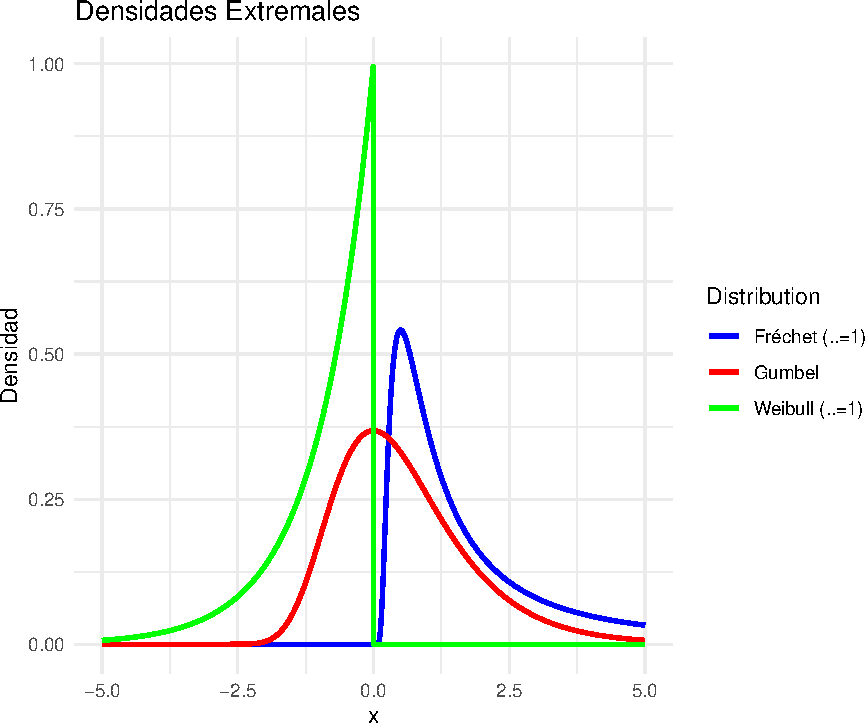
\includegraphics{_main_files/figure-latex/plot-extreme-distributions-1.pdf}

A estas versiones standard se las puede extender
agregando un parámetro de recentramiento \((\mu)\) y
un parámetro de escala \((\beta)\).

Se dice que \(X\) tiene distribución:

\begin{itemize}
\item
  \(\Lambda^{(\mu, \beta)}\) si \(\;X=\mu + \beta Y\;\), donde \(Y\) tiene distribución \(\Lambda\).
\item
  \(\;\Psi^{(\mu, \beta)}\;\) si \(\;X=\mu + \beta Y\;\), donde \(Y\) tiene distribución \(\Psi_{\alpha}\).
\item
  \(\;\Phi^{(\mu, \beta)}\;\) si \(X=\mu + \beta Y\), donde \(Y\) tiene distribución \(\Phi_{\alpha}\).
\end{itemize}

En general, es en este sentido que diremos que una
variable es Gumbel, Weibull o Fréchet (incluyendo
recentramiento y reescalamiento), pero en cálculos
donde los parámetros \(\mu\) y \(\beta\) no sean relevantes, por
simplicidad, usaremos las versiones standard.

El siguiente teorema vincula las distribuciones
extremales en sus formatos standard y resulta de
gran utilidad práctica sobre todo al hacer tests de
ajustes, etc.

\textbf{Teorema 1 : \emph{Relaciones entre las versiones
standard de las distribuciones extremales.}}

\begin{Shaded}
\begin{Highlighting}[]
\SpecialCharTok{{-}}\FunctionTok{digamma}\NormalTok{(}\DecValTok{1}\NormalTok{) }\CommentTok{\# Constante de Euler{-}Mascheroni}
\end{Highlighting}
\end{Shaded}

\begin{verbatim}
## [1] 0.5772157
\end{verbatim}

\begin{Shaded}
\begin{Highlighting}[]
\FunctionTok{mean}\NormalTok{(}\FunctionTok{rgumbel}\NormalTok{(}\DecValTok{1000}\NormalTok{))}
\end{Highlighting}
\end{Shaded}

\begin{verbatim}
## [1] 0.5893328
\end{verbatim}

\begin{Shaded}
\begin{Highlighting}[]
\FunctionTok{sd}\NormalTok{(}\FunctionTok{rgumbel}\NormalTok{(}\DecValTok{1000}\NormalTok{))}
\end{Highlighting}
\end{Shaded}

\begin{verbatim}
## [1] 1.257799
\end{verbatim}

\subsubsection{Distribución de Weibull}\label{distribuciuxf3n-de-weibull}

Se dice que una variable tiene distribución de
Weibull de orden \(\alpha>0\) si su distribución es:

\[\Psi_{\alpha}(x)=\begin{cases}
exp{-(-x)^{\alpha}} & si\;x<0\\
1 & \text{en otro caso}
\end{cases}\]
Recordemos que cuando tomamos los máximos de las variables \(iid\) con un rango acotado, la distribución resultante por la cual se puede aproximar es la de Weibull. En este caso, y en el resto del LAB, exp() y e son la función exponencial.

Por una única vez, calculemos la distribución de forma ``manual'' en el R para convencernos de la forma de la función de distribución de Weibull (\(\Psi\)). Para eso generaremos un vector auxiliar de valores \(x\) y la distribución (\(F(x)\)). En R la definición de la distribución es sutilmente diferente a la que vimos en el teórico (definida para positivos), pero totalmente convertible con dos cambios de signo. La función que calcula la probabilidad de una distribución Weibull es \textbf{pweibull()}. Pueden ver la definición de R utilizando help(pweibull) o ?pweibull.En R podemos saber la forma y valores de esta distribución con una función implementada en un paquete base \{stats\}. La función es pweibull y lleva como argumentos un vector de cuantiles ( q ), un argumento de forma ( shape ) y otro de escala ( scale ). Recordemos que la función plot utiliza 2 argumentos centrales ( x e y ) y podemos fijar los límites del gráfico ( xlim e ylim), el tipo de gráfico ( type) y las etiquetas de los ejes X e Y ( xlab e ylab).

Primero generaremos un vector de numeros auxiliares equiespaciados y lo nombraremos (``x\_aux''). Luego definiremos un orden (alpha=α
) de la Weibull y graficaremos la función.

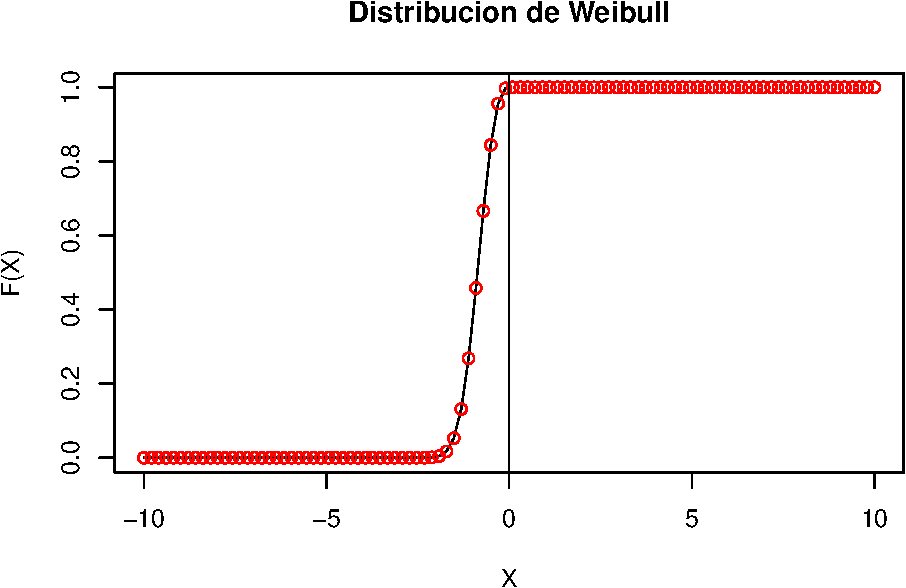
\includegraphics{_main_files/figure-latex/unnamed-chunk-7-1.pdf}
Veamos ahora la forma de un par de distribuciones cambiando el parámetro de orden (α
), que en la función pweibull de R se nombra como shape y que define el orden de la distribución.

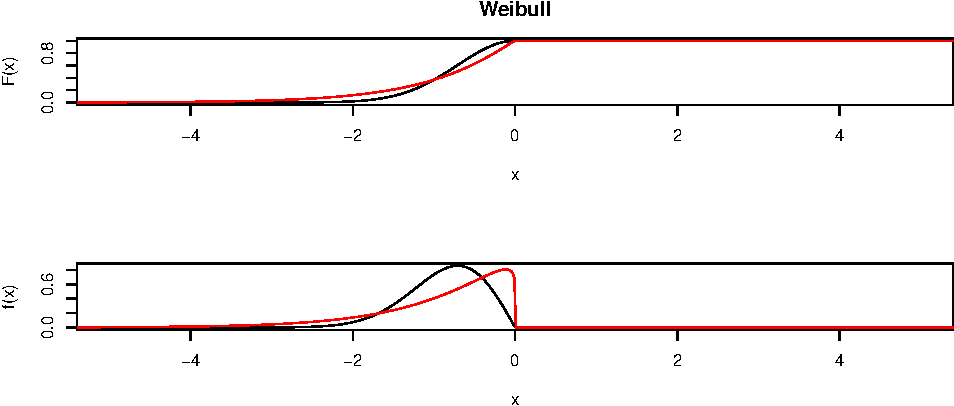
\includegraphics{_main_files/figure-latex/unnamed-chunk-8-1.pdf}
En R podemos también generar numeros aleatórios (técnicamente pseudo-aleatorios) de una distribución extremal. Estos simuladores de números aleatórios son útiles para comparar contra distribuciones nulas, generar modelos sintéticos para probar algorítmos, etc\ldots{}
Para lxs que venimos de la rama mas aplicada, muchas veces nos ayudan a entender como funcionan los modelos y a verificar si nuestra intuición es acertada respecto a la escala de ajuste de los parámetros entre otras útiles. Generaremos 2 series de 1000 números aleatórios con la función rweibull, que tiene como parámetro el número de datos que se necesitan y la forma (shape) de la distribución. Luego haremos un grafico con la densidad empírica (esto es similar a un histograma) de estos vectores.

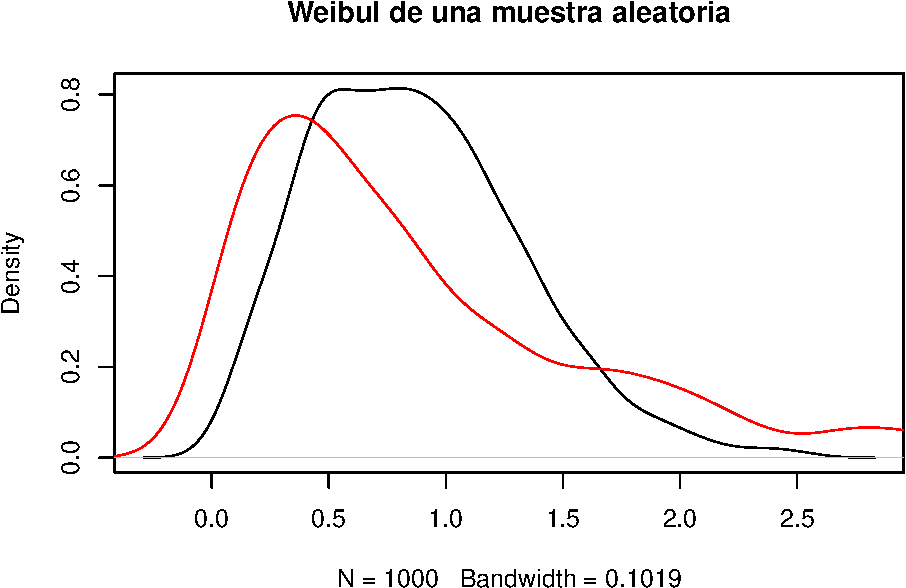
\includegraphics{_main_files/figure-latex/unnamed-chunk-9-1.pdf}

\subsubsection{Distribución de Fréchet}\label{distribuciuxf3n-de-fruxe9chet}

Se dice que una variable tiene distribución de
Fréchet de orden \(\alpha>0\) si su distribución es:

\[
\Phi_{\alpha}(x)=\begin{cases}
exp\{-x^{-\alpha}\} & si\;x>0\\
0 & \text{en otro caso}
\end{cases}
\]

Esta tercera clase de variables incluyen a las distribuciones no acotadas, pero de colas pesadas. Es decir que tienen una probabilidad alta de presentar valores alejados de la media o la mediana (ej. la Cauchy). En estos casos, la distribución de sus máximos es la Frechet. Grafiquemos esta distribución para dos valores diferentes de \(\alpha\).

\begin{Shaded}
\begin{Highlighting}[]
\NormalTok{x\_aux}\OtherTok{\textless{}{-}} \FunctionTok{seq}\NormalTok{(}\SpecialCharTok{{-}}\DecValTok{10}\NormalTok{,}\DecValTok{10}\NormalTok{, }\AttributeTok{length=}\DecValTok{1000}\NormalTok{)}

\FunctionTok{par}\NormalTok{(}\AttributeTok{mfrow=}\FunctionTok{c}\NormalTok{(}\DecValTok{3}\NormalTok{,}\DecValTok{1}\NormalTok{), }\AttributeTok{mar=}\FunctionTok{c}\NormalTok{(}\DecValTok{5}\NormalTok{,}\DecValTok{4}\NormalTok{,}\DecValTok{3}\NormalTok{,}\DecValTok{1}\NormalTok{))}
\FunctionTok{plot}\NormalTok{(}\FunctionTok{seq}\NormalTok{(}\SpecialCharTok{{-}}\DecValTok{10}\NormalTok{,}\DecValTok{10}\NormalTok{,}\AttributeTok{length=}\DecValTok{100}\NormalTok{), }\FunctionTok{pfrechet}\NormalTok{(}\AttributeTok{q=}\FunctionTok{seq}\NormalTok{(}\SpecialCharTok{{-}}\DecValTok{10}\NormalTok{,}\DecValTok{10}\NormalTok{,}\AttributeTok{length=}\DecValTok{100}\NormalTok{), }\AttributeTok{shape=}\DecValTok{2}\NormalTok{, }\AttributeTok{scale=}\DecValTok{1}\NormalTok{) ,}\AttributeTok{xlim=}\FunctionTok{c}\NormalTok{(}\SpecialCharTok{{-}}\DecValTok{2}\NormalTok{,}\DecValTok{10}\NormalTok{), }\AttributeTok{type=}\StringTok{"l"}\NormalTok{, }\AttributeTok{ylab=}\StringTok{"F(x)"}\NormalTok{, }\AttributeTok{xlab=}\StringTok{"x"}\NormalTok{, }\AttributeTok{main=}\StringTok{"Frechet"}\NormalTok{)}
\FunctionTok{lines}\NormalTok{(}\FunctionTok{seq}\NormalTok{(}\SpecialCharTok{{-}}\DecValTok{10}\NormalTok{,}\DecValTok{10}\NormalTok{,}\AttributeTok{length=}\DecValTok{100}\NormalTok{), }\FunctionTok{pfrechet}\NormalTok{(}\AttributeTok{q=}\FunctionTok{seq}\NormalTok{(}\SpecialCharTok{{-}}\DecValTok{10}\NormalTok{,}\DecValTok{10}\NormalTok{,}\AttributeTok{length=}\DecValTok{100}\NormalTok{), }\AttributeTok{shape=}\FloatTok{1.1}\NormalTok{, }\AttributeTok{scale=}\DecValTok{1}\NormalTok{),}\AttributeTok{col=} \StringTok{"red"}\NormalTok{)}

\FunctionTok{plot}\NormalTok{(x\_aux, }\FunctionTok{dfrechet}\NormalTok{(}\AttributeTok{x=}\NormalTok{x\_aux, }\AttributeTok{shape=}\DecValTok{2}\NormalTok{, }\AttributeTok{scale=}\DecValTok{1}\NormalTok{, }\AttributeTok{log =} \ConstantTok{FALSE}\NormalTok{) ,}\AttributeTok{xlim=}\FunctionTok{c}\NormalTok{(}\SpecialCharTok{{-}}\DecValTok{2}\NormalTok{,}\DecValTok{10}\NormalTok{), }\AttributeTok{type=}\StringTok{"l"}\NormalTok{, }\AttributeTok{ylab=}\StringTok{"f(x)"}\NormalTok{, }\AttributeTok{xlab=}\StringTok{"x"}\NormalTok{)}
\FunctionTok{lines}\NormalTok{(x\_aux, }\FunctionTok{dfrechet}\NormalTok{(}\AttributeTok{x=}\NormalTok{x\_aux, }\AttributeTok{shape=}\FloatTok{1.1}\NormalTok{, }\AttributeTok{scale=}\DecValTok{1}\NormalTok{, }\AttributeTok{log =} \ConstantTok{FALSE}\NormalTok{), }\AttributeTok{col=}\StringTok{"red"}\NormalTok{)}
\end{Highlighting}
\end{Shaded}

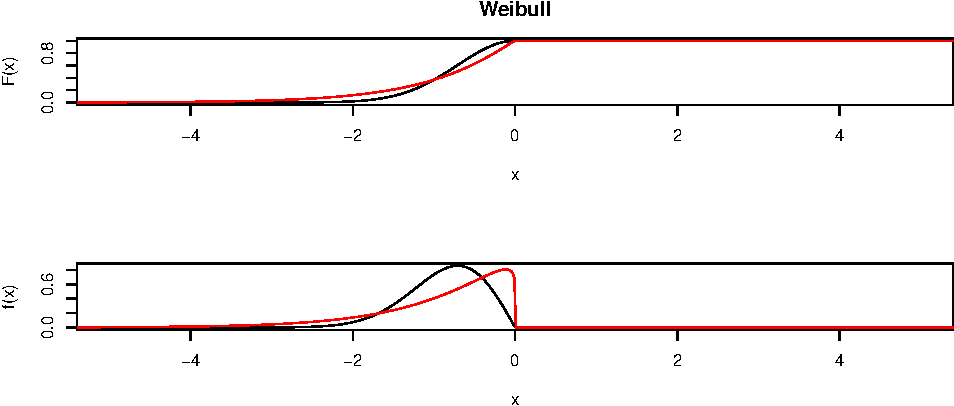
\includegraphics{_main_files/figure-latex/unnamed-chunk-10-1.pdf}

.

\newpage

\paragraph{Teorema 1: Relaciones entre las versiones standard de las distribuciones extremales}\label{teorema-1-relaciones-entre-las-versiones-standard-de-las-distribuciones-extremales}

\(X\) tiene distribución \(\Phi_{\alpha}(x)\) si y sólo si \((-1/X)\) tiene
distribución \(\Psi_{\alpha}(x)\) si y sólo si \(log(X^{\alpha})\) tiene
distribución \(\Lambda\).

\paragraph{Teorema 2: Algunos datos de las distribuciones extremales}\label{teorema-2-algunos-datos-de-las-distribuciones-extremales}

\paragraph{Parte 1}\label{parte-1}

Si \(X\) tiene distribución \(\Lambda^{(\mu,\beta)}\) entonces tiene:

\begin{itemize}
  \item[a)] Valor esperado: $E(X) = \mu + \beta\gamma$, donde $\gamma$ es la constante de Euler-Mascheroni, cuyo valor aproximado es $0.5772156649$.
  \item[b)] Moda: $\mu$
  \item[c)] Mediana: $\mu - \beta \log(\log 2) \approx \mu - 0.36651 \beta$.
  \item[d)] Desviación estándar: $\beta \pi \sqrt{6} \approx 1.2825 \beta$.
  \item[e)] Si $X^+ = \max(X,0)$, entonces $E(X+k)$ es finito para todo valor de $k$ natural.
  \item[f)] Para simular computacionalmente $X$, se puede tomar $U$ uniforme en $(0,1)$ y hacer $X = \mu - \beta \log(-\log U)$.
\end{itemize}

\subsubsection{Parte 2}\label{parte-2}

Si \(X\) tiene distribución \(\Psi_{\alpha}^{(\mu,\beta)}\) entonces tiene:

\begin{itemize}
  \item[a)] Valor esperado: $E(X) = \mu + \beta\Gamma(1+1/\alpha)$.
  \item[b)] Moda: $\mu$ si $\alpha\leq 1$ y $\mu-\beta\{(\alpha-1)/\alpha\}^{(1/\alpha)}$ si $\alpha>1$.
  \item[c)] Mediana: $\mu - \beta \log(2)^{(1/\alpha)}$.
  \item[d)] Desviación estándar: $\beta\{\Gamma(1+2/\alpha)-\Gamma(1+1/\alpha)^2\}^{1/2}$.
\end{itemize}

\subsubsection{Parte 2}\label{parte-2-1}

Si \(X\) tiene una distribución \(\Phi_{\alpha}^{(\mu, \beta)}\) entonces se tiene:

\begin{itemize}
  \item[a)] Valor esperado: $E(X) = \mu + \beta\Gamma(1-1/\alpha)$ si $\alpha > 1$, $\infty$ en caso contrario.
  \item[b)] Moda: $\mu + \beta\Gamma(1-1/\alpha)$ si $\alpha>1$.
  \item[c)] Mediana: $\mu + \beta \log(2)^{(-1/\alpha)}$.
  \item[d)] Desviación estándar: $\beta|\Gamma(1-2/\alpha)-\Gamma(1-1/\alpha)^2|$ si $\alpha>2$, $\infty$ si $1<\alpha \leq 2$.
\end{itemize}

\newpage

\paragraph{Teorema 3: Fischer-Tippet-Gnedenko (FTG)}\label{teorema-3-fischer-tippet-gnedenko-ftg}

Si \(X_1,...,X_n\quad iid\) con distribución \(F\) ``continua'', llamamos \(F_n^*\) a la distribución de \(max(X_1,...,X_n)\) y \(n\) es grande, entonces existen \(\mu\) real y \(\beta>0\) tales que alguna de las siguientes tres afirmaciones es correcta:

\begin{itemize}
  \item[1)] $F_n^*$ se puede apromixar por la distribución de $\mu+\beta Y$ con $Y$ variable con distribución $\Lambda$.
  \item[2)] Existe $\alpha>0$ tal que $F_n^*$ se puede aproximar por la distribución de $\mu+\beta Y$ con $Y$ variable con distribución $\Phi_{\alpha}$. 
  \item[3)] Existe $\alpha>0$ tal que $F_n^*$ se puede aproximar por la distribución de $\mu+\beta Y$ con $Y$ variable con distribución $\Phi_{\alpha}$.
\end{itemize}

Lo anterior equivale a decir que la distribución del máximo de datos \textit{continuos} e \(iid\), si \(n\) es grande, puede aproximarse por una Gumbel, una Fréchet o una Weibull. Una aproximación será válida dependiendo de la distribución de \(F\). En este sentido, cuando \(F\) sea normal entonces \(F_n^*\) se puede aproximar como una Gumbel. Cuando \(F\) sea uniforme, se puede aproximar \(F_n^*\) como una Weibull y cuando \(F\) sea Cauchy entonces \(F_n^*\) se puede aproximar por una Fréchet.

Más precisamente, cuál de las tres aproximaciones es la aplicable depende de la cola de \(F\) (los valores de \(F(t)\) para valores grandes de \(t\)).
En concreto, Weibull aparece cuando \(F\) es la distribución de una variable acotada por arriba (como la Uniforme), Gumbel para distribuciones de variables no acotadas por arriba pero con colas muy livianas (caso Exponencial y Normal) y Fréchet para colas pesadas (caso Cauchy)\footnote{Si bien  la hipótesis de continuidad de $F$ no es esencial, si $F$ tiene
la distribución Binomial o Poisson, por ejemplo, no se puede aplicar ninguna de las tres aproximaciones anteriores.}.

Como consecuencia del \(FTG\) cuando se tengan datos máximos, las distribuciones maximales podrían ser candidatas de uno de los ajustes si

\begin{itemize}
\item la cantidad de registros es lo suficientemente grande
\item los registros son $iid$ aunque con versiones más generales del $FTG$ este supuesto puede no cumplirse
\end{itemize}

Como la mayoría de tests de ajustes suponen datos \(iid\), se van a realizar dos tests de aleatoriedad\footnote{En inglés se expresa como \textit{randomness}} a los datos:

\begin{itemize}
\item  Runs up and down 
\item  Spearman correlation of ranks 
\end{itemize}

Se emplea la prueba de ajuste \(\chi^2\) que requiere seleccionar una partición más o menos arbitraria de la recta real de intervalos siendo importante que en cada intervalo haya una cantidad lo suficientemente importante de datos de la muestra. En este sentido, se pueden tomar como extremos de los intervalos los quintiles empíricos de la muestra. Cabe mencionar que este test requiere estimar parámetros por el método de Máxia Verosimilitud Categórica.

Cabe mencionar que para este estudio la distribución de la variable a incorporar en este estudio no tiene que ser degenerada, es decir \(H(t)=0\) ó \(H(t)=1\).

\newpage

\subsection{Definición 2: Distribución extremal asintótica}\label{definiciuxf3n-2-distribuciuxf3n-extremal-asintuxf3tica}

Si \(X_1,...,X_n\) es \(iid\) con distribución \(F\) diremos que \(H\) no-degenerada es la Distribución Extremal Asintótica (DEA) de \(F\)\footnote{Lo que equivale a decir que $F$ tiene $DEA\;H$.}, si existen dos sucesiones de números reales, \(d_n\) y \(c_n>0\), tales que la distribución de

\begin{equation}
\frac{max(X_1,...,X_n)- d_n}{c_n}\label{eq:max}
\end{equation}

tiende a \(H\) cuando \(n\) tiende a infinito.

\subsection{Definición 3: Supremo esencial de una variable aleatoria o distribución}\label{definiciuxf3n-3-supremo-esencial-de-una-variable-aleatoria-o-distribuciuxf3n}

Si \(X\) tiene distribución \(F\), se llama supremo esencial de \(X\), denotado como \(M_X\) o, indistintamente, supremo esencial de \(F\), denotado \(MF\) a

\begin{equation}
M_X=M_F= sup\{t / F(t)<1\}\label{eq:Mx}
\end{equation}

Observación:

\begin{itemize}
\item Si $F$ es $U(a,b)$, $M_F=b$
\item Si $F$ es $Bin(m,p)$, $M_F=m$
\item Si $F$ es Normal, Exponencial, Cauchy o Poisson, $M_F$ es infinito.
\end{itemize}

\paragraph{Teorema 4}\label{teorema-4}

Si \(X_1,...,X_n\) es \(iid\) con distribución \(F\) cualquiera, entonces, para \(n\) tendiendo a infinito,

\begin{equation}
X^*_n=M_F= max(X_1,...,X_n)\;tiende\;a\;M_F\label{eq:Xast}
\end{equation}

Observación:

El resultado anterior vale incluso si \(M_F\) es infinito, pero si \(M_F\) es finito, como \(X^*n - M_F\) tiende a cero, por analogía con el Teorema Central del Límite para promedios, buscaríamos una sucesión \(c_n>0\) y que tienda a cero de modo tal que \((X^*n- M_F )/ c_n\) tienda a una distribución no-degenerada y de allí surge buscar la DEA.

\paragraph{Teorema 5}\label{teorema-5}

Si \(F\) es una distribución con \(M_F\) finito, y para \(X\) con distribución \(F\) se cumple que

\[
P(X=M_F)>0 
\]

entonces \(F\) NO admite DEA.

Observación:

Si \(F\) es \(Bin(m,p)\), \(M_F=m\). Si \(X\) tiene distribución \(F\), entonces
\(P( X=M_F)= P( X=m)= p_m>0\),
asi que la distribucion \(Bin(m,p)\) NO admite DEA, no se puede aproximar la distribución del máximo de una muestra \(iid\) de variables \(Bin(m,p)\).

El Teorema anterior es un caso particular del próximo.

\paragraph{Teorema 6}\label{teorema-6}

Si \(F\) es una distribución con \(M_F\) finito o infinito que admite DEA, y \(X\) tiene distribución \(F\), entonces el límite cuando \(t\) tiende a \(M_F\) por izquierda de
\(P(X>t)/P(X \geq t)\) debe ser 1.

Observación:

\begin{itemize}
\item Si $F$ es una distribución de Poisson de parámetro $\lambda>0$, $M_F$ es infinito. 
\item Si $k$ es un natural, entonces:
\begin{eqnarray}
\frac{P(X>k)}{P(X\geq k)} &=& \frac{P(X \geq k+1)}{P(X\geq k)} \\ \nonumber
&=& 1-\frac{P(X=k)}{P(X \geq k)} \approx 1-\left(1- \frac{\lambda}{k}\right) 
\end{eqnarray}
que tiende a $0$ cuando $k$ tiende a infinito, por lo cual $F$ NO admite DEA, o sea que no se puede aproximar el máximo de una sucesión $iid$ de variables de Poisson.
\end{itemize}

Observación:

El Teorema 6 brinda una condición NECESARIA pero NO SUFICIENTE para DEA. Un ejemplo de ello lo aportó Von Mises, mostrando que la distribución

\[F(x)= 1- e^{(-x-sen(x))}\]
cumple con la condicion del Teorema 6 pero no admite DEA.

\subsection{Definición 4: Distribución max-estables}\label{definiciuxf3n-4-distribuciuxf3n-max-estables}

Si dada una \(F\) distribución, \(X\) con distribución \(F\), \(k\) natural arbitrario y \(X_1,...,X_k\) es \(iid\) con distribución \(F\), existen reales \(a_k\), \(b_k\) tales que \(max(X_1,...,X_k)\) tiene la misma distribución que \(a_k X+ b_k\), \(F\) se dice \textit{max-estable}.

El Teorema FTG resulta de superponer los dos siguientes teoremas:

\paragraph{Teorema 7}\label{teorema-7}

\begin{itemize}
  \item[a)] Si $F$ admite $DEA\;H$, entonces $H$ es max-estable.
  \item[b)] Si $H$ es max-estable, es la DEA de sí misma.
\end{itemize}

\paragraph{Teorema 8}\label{teorema-8}

Una distribución es max-estable si y solo si es extremal\footnote{O sea Gumbel, Weibull o Fréchet}.
El Teorema 7 es bastante intuitivo y análogo a los teoremas de Lévy sobre distribuciones estables en aproximaciones asintóticas de las distribuciones de sumas. Para el Teorema 8 haremos enseguida un ejercicio sencillo que nos ayudará a hacerlo creíble.
Luego precisaremos, para terminar con esta parte, cómo son las distribuciones que tienen por DEA cada uno de los tres tipos de distribuciones extremales. Para eso precisamos recordar algunas definiciones, como la siguiente.

Obsrvación:

Si \(F\) y \(G\) son dos distribuciones, tienen colas equivalentes si \(M_F=M_G\) y cuando \(t\) tiende a \(M_F\) por izquierda, \((1-F(t))/(1-G(t))\) tiende a un valor \(c>0\).
Recordando ahora cómo se calcula la distribución del máximo de dos variables independientes, es muy sencillo calcular la distribución del \(max\{X,Y\}\), cuando \(X\) e \(Y\) son independientes y cada una de ellas es una distribución extremal.

Se tiene el siguiente resultado:

\begin{longtable}[]{@{}
  >{\raggedright\arraybackslash}p{(\columnwidth - 4\tabcolsep) * \real{0.2500}}
  >{\raggedright\arraybackslash}p{(\columnwidth - 4\tabcolsep) * \real{0.2500}}
  >{\raggedright\arraybackslash}p{(\columnwidth - 4\tabcolsep) * \real{0.5000}}@{}}
\toprule\noalign{}
\begin{minipage}[b]{\linewidth}\raggedright
\(X\)
\end{minipage} & \begin{minipage}[b]{\linewidth}\raggedright
\(Y\)
\end{minipage} & \begin{minipage}[b]{\linewidth}\raggedright
\(max(X,Y)\)
\end{minipage} \\
\midrule\noalign{}
\endhead
\bottomrule\noalign{}
\endlastfoot
\textcolor{red}{Weibull} & \textcolor{red}{Weibull} & \textcolor{red}{Weibull} \\
\textcolor[rgb]{0.0,0.5,0.0}{Weibull} & \textcolor[rgb]{0.0,0.5,0.0}{Gumbel} & \textcolor[rgb]{0.0,0.5,0.0}{Cola equivalente Gumbel} \\
\textcolor{blue}{Weibull} & \textcolor{blue}{Fréchet} & \textcolor{blue}{Fréchet} \\
\textcolor[rgb]{0.0,0.5,0.0}{Gumbel} & \textcolor[rgb]{0.0,0.5,0.0}{Weibull} & \textcolor[rgb]{0.0,0.5,0.0}{Cola equivalente Gumbel} \\
\textcolor{red}{Gumbel} & \textcolor{red}{Gumbel} & \textcolor{red}{Gumbel} \\
\textcolor{blue}{Gumbel} & \textcolor{blue}{Fréchet} & \textcolor{blue}{Cola equivalente Fréchet} \\
\textcolor{blue}{Fréchet} & \textcolor{blue}{Weibull} & \textcolor{blue}{Fréchet} \\
\textcolor{blue}{Fréchet} & \textcolor{blue}{Gumbel} & \textcolor{blue}{Cola equivalente Fréchet} \\
\textcolor{red}{Fréchet} & \textcolor{red}{Fréchet} & \textcolor{red}{Fréchet} \\
\end{longtable}

\textcolor{red}{\rule{1em}{1em} Las extremales son max-estables: tomar máximos de dos del mismo tipo queda en el mismo tipo.}

\textcolor[rgb]{0.0,0.5,0.0}{\rule{1em}{1em} Gumbel es más pesada que Weibull. En la cola, que es lo que cuenta para máximos, prima Gumbel.}

\textcolor{blue}{\rule{1em}{1em} Fréchet es más pesada que Gumbel y mucho más pesada que Weibull.}
\vspace{1cm}

Además, de la tabla se deduce que

\paragraph{Teorema 9}\label{teorema-9}

Si \(X_1,...,X_n\) independientes y cada \(X_i\) tiene uno de los tres tipos de distribución extremal, entonces la distribución del \(max(X_1,...,X_n)\) es:

\begin{itemize}
\item[a)] Cola equivalente a Fréchet, si alguna de las variables es Fréchet y alguna otra es Gumbel.
\item[b)]  Fréchet, si alguna es Fréchet y ninguna es Gumbel.
\item[c)]  Cola equivalente Gumbel ninguna es Fréchet pero algunas son Gumbel y otras Weibull.
\item[d)] Gumbel si todas son Gumbel.
\item[e)]  Weibull si todas son Weibull.
\end{itemize}

Observación:

Si \(F\) es una distribución, se dice que tiene \textit{cola de variación regular de orden} \(-\alpha\), para \(\alpha \geq 0\), si para todo \(t>0\), \((1-F(tx))/(1-F(x))\) tiende
a \(t^{-\alpha}\) si \(x \rightarrow  \infty\). Para abreviar se dirá que \(F\) es \(R_{-\alpha}\). Por ejemplo, para \(\alpha=3\), un caso de una tal \(F\) es \(F(u)=1- 1/u^3\).

Por otra parte se dice que \(L\) es una \textit{función de variación lenta} si, para todo \(t>0\), \(L(tx)/L(x)\) tiende a 1 cuando \(x \rightarrow  \infty\). Por ejemplo, \(L(u)=log(u)\).

\newpage

\subsection{Definición 4: Dominio de atracción maximal}\label{definiciuxf3n-4-dominio-de-atracciuxf3n-maximal}

Si \(H\) es una distribución extremal (Gumbel, Weibull o Fréchet) su Dominio de Atracción Maximal (\(DAM(H)\)) está constituído por todas las distribuciones \(F\) que tienen \(DEA\;H\).

\paragraph{Teorema 9: DAM de la Fréchet}\label{teorema-9-dam-de-la-fruxe9chet}

\(F\) pertenece a la DAM de \(\Phi_{\alpha}\) si y sólo si
\(1-F(x)=x-\alpha L(x)\) para alguna \(L\) de variación lenta,
lo cual es equivalente a decir que \(F\) es \(R_{-\alpha}\).

\paragraph{Corolario 1: DAM de la Fréchet}\label{corolario-1-dam-de-la-fruxe9chet}

Si \(F\) es una distribución con densidad \(f\) que cumple que \(xf(x)/(1-F(x))\) tiende a \(\alpha\) cuando \(x \rightarrow  \infty\)
se dice que \(F\) cumple la Condición de Von Mises I. En tal caso, \(F\) pertenece a la DAM de \(\Phi_{\alpha}\) y mas aún, la DAM de \(\Phi_{\alpha}\) son todas las distribuciones que tienen cola equivalente a alguna distribución que cumpla la Condición de Von Mises I.
Del DAM Fréchet y Teorema 1, surge lo siguiente.

\paragraph{Teorema 10: DAM de la Weibull}\label{teorema-10-dam-de-la-weibull}

\begin{itemize}
\item [a)] $F$ pertenece a la DAM de $\Psi_{\alpha}$ si y solo si $M_F$ es finito y además $$1-F(M_F -1/x)=x^{-\alpha} L(x)$$ para alguna
$L$ de variación lenta, es decir que pertenece a $R_{-\alpha}$. Observar que con el cambio de variable $u=M_F -1/x$,
resulta que $1-F(u)=(^{-}MF -u)^{\alpha} L(1/(M_F -u))$ para alguna $L$ de variación lenta, para $u< M_F$. Además puede tomarse $d_n= M_F$ y $c_n= n-\alpha$.
\item [b)] Si $F$ distribución con densidad $f$ positiva en $(a,M_F)$ para algun $a< M_F$ y $(M_F -x)f(x)/(1-F(x))$ tiende a $\alpha$ cuando $x\rightarrow M_F$, se dice que $F$ cumple la Condición de Von Mises II. En tal caso $F$ pertenece a la DAM de $\Psi_{\alpha}$ y mas aún, la DAM de $\Psi_{\alpha}$ son todas las distribuciones que tienen cola equivalente a alguna distribución que cumpla la Condición de Von Mises II.
\end{itemize}

\paragraph{Teorema 11: DAM de la Gumbel}\label{teorema-11-dam-de-la-gumbel}

Una distribución \(F\) se dice una Función de Von Mises con función auxiliar \(h\) si existe \(a < M_F\) (\(M_F\) puede ser finito o infinito) tal que para algún \(c>0\) se tiene

\[
1-F(x)= c\;exp^{{- \int_a^X \frac{1}{h(t)} dt}},
\]

con \(h\) positiva, con
densidad \(h^\prime\) y \(h^\prime(x)\) tendiendo a \(0\) para \(x\rightarrow M_F\)
Se tiene entonces que la \(DAM\) de \(\Lambda\) son todas las distribuciones que tienen cola equivalente a alguna distribución que sea una Función de Von Mises. Básicamente, se trata de colas más livianas que cualquier expresión del tipo \(1/x^k\), más aún, con decaimiento \textit{del tipo exponencial}, en el sentido preciso siguiente: si como en el Teorema 11

\(1-F(x)= c\;exp^{{- \int_a^X \frac{1}{h(t)} dt}}\), entonces se tiene
\(1-F(x)= c\;exp^{-(x-a)/h(x)}\), donde la función auxiliar \(h\) es no-decreciente y con asíntota horizontal.

Además, \(d_n\) y \(c_n\) suelen involucrar expresiones logarítmicas. Más concretamente, \(dn = F^{-1}(1-1/n)\),
\(c_n = h(d_n)\), donde \(F^{-1}\) es la inversa generalizada (o función cuantil), definida por
\(F^{-1}(p)= inf\{t / F(t)\geq p\}\), para \(0<p<1\).

\subsection{Corolario 2 :}\label{corolario-2}

Si \(F\) pertenece al \(DAM\) Gumbel, \(M_F\) es infinito, y se considera \(X\) con distribucion \(F\), entonces \(E(X+k)\) es finito para todo \(k\) natural.
Los resultados antes vistos nos permiten reconocer que distribuciones tienen \(DEA\) y si la tienen, cual es. Cierran el tema. Adicionalmente, permiten ver con mucha precision que el quid de esta teoría es el comportamiento de las colas de las distribuciones, que Fréchet corresponde a las colas más pesadas, luego la Gumbel y finalmente Weibull.
Para terminar el capítulo presentaremos la distribución de valores extremos generalizada\footnote{GEV, por sus siglas en inglés.}, que es una forma de compactar en una unica fórmula las tres distribuciones extremales, debida a Jenkinson-Von Mises.

\subsection{Definición 5: GEV}\label{definiciuxf3n-5-gev}

Se define a la distribución de valores extremos generalizada \((GEV)\)\footnote{Por sus siglas en inglés relativas a Generalized Extreme Values.} de posición \(\mu\), escala \(\beta\) e índice \(\xi\) con

\[
G(\mu,\beta,\xi) =
\begin{cases}
    e^{-(1+ \xi(t-\mu)/ \beta)(-1/ \xi)} & \text{si  } \xi \neq 0, \forall\;t\;\text{donde } 1+ \xi(t-\mu)/ \beta) >0 \\
    e^{-e^{(-(t-\mu)/ \beta)}} & \text{si  } \xi =0,\; \forall \;t \\
\end{cases}
\]
\vspace{0.5cm}

En los casos en que \(\xi\) tome los siguientes valores, se tiene

\begin{align*}
 \xi=0,  & \text{ corresponde a Gumbel,} \\
 \xi< 0, &\text{ corresponde a Weibull y } \alpha=-1/ \xi \\
 \xi>0, &\text{ corresponde Fréchet y }  \alpha=1/ \xi
\end{align*}

En \(R\) existen rutinas para estimar \(\xi\) con intervalos de confianza( por máxima verosimilitud, etc.) lo cual da formas de testear si una extremal es Gumbel, Weibull o Fréchet.

Observación:

En algunas situaciones datos extremales pueden ajustarse a más de un modelo. Por ejemplo, puede ocurrir que tanto ajusten los datos una Gumbel como una Weibull. Frente a estas situaciones, no hay una receta única de cómo proceder sino que quien está modelando debe tener claro si corresponde volcarse hacia cálculos más pesimistas (que dan mayor probabilidad a eventos extremos muy severos) o más optimistas.

Usualmente la opción pesimista implica privilegiar la seguridad y la optimista la economía de recursos, pero insistimos en que la reflexión ante cada caso es indispensable. Un poquito más adelante veremos, al comparar un modelo Gumbel con un modelo Fréchet, que las diferencias pueden ser sumamente drásticas.

Observación:

Antes de seguir adelante, demos la respuesta a la parte \(a)\) del Ejercicio 5. Es un ejercicio de Cálculo Diferencial sencillo mostrar que la cola de un \(N(0,1)\), es decir \(Q(t)=P(X>t)\), donde \(X\) tiene distribución \(N(0,1)\), es equivalente, para \(t\) tendiendo a infinito, a la función \(\phi(t)/t\), donde \(\phi\) representa la densidad normal típica (campana de Gauss). Basándose en esto, si se considera ahora una variable log-normal \(Y\), tal que \(log(Y)\) es una \(N(0,1)\), puede probarse que su cola \(R(t)=P(Y>t)\), es equivalente, para \(t\) tendiendo a infinito, a la función \(\phi(log(t))/log(t)\). Con un poco más de Cálculo, esta última función puede escribirse para \(a>e\) (por ejemplo \(a=3\)), como

\begin{equation}
c\times e^{-\int_{a}^{t}1/h(s)\; ds} \quad \text{para }\: t>a
\end{equation}

donde \(c\) se expresa en función de \(a\) y \(h(s)=\frac{s\; log(s)}{(log(s))^2+1}\) la cual cumple las hipótesis del Teorema 11.

Se concluye entonces que la log-normal está en el \(DAM\) Gumbel, o lo que es lo mismo, que la log- normal admite \(DEA\) Gumbel.

Observación: Tiempos y Valores de Retorno

En Ingeniería y Ciencias Ambientales, suele pensarse los eventos extremos (por ejemplo: observación por encima de cierto valor muy alto), en términos de tiempos de retorno (tiempo que se espere para que ocurra un evento). Bajo las hipótesis de datos \(iid\), el tiempo de retorno \(T\) tiene una distribución \(Geo(p)\), con \(p = P(evento)\), por lo cual el tiempo de retorno medio es \(E(T)=1/p\) y pueden hacerse intervalos de confianza para \(E(T)\), en la medida que exista información de \(P(evento)\), lo cual puede obtenerse a partir de este capítulo o de los siguientes. Cabe observar que muchas veces se utiliza la expresión Tiempo de Retorno (TR) para \(E(T)\).

Más precisamente, \(TR(u)\), el Tiempo de retorno del valor \(u\), es el valor esperado (o la media) del tiempo que se debe esperar para que la variable en estudio supere el valor \(u\), es decir que \(TR(u) = 1/P(X>u)\), si \(X\) es la variable en estudio.

Por otro la lado, en una mirada inversa, el Valor de Retorno a tiempo \(t\), \(VR(t)\) es el valor de \(u\) para el cual \(TR(u)=t\), es decir que \(TR(VR(t))=t\) (y también \(VR(TR(u))=u\), es decir que \(TR\) y \(VR\) son, como funciones, inversas una de la otra).

Para \textit{bajar un poco a tierra} estos conceptos, vamos a calcularlos y compararlos cuando la variable \(X\) es Gumbel y cuando (con los mismos valores de posición \(\mu\) y escala \(\beta>0\)).

Comencemos por la Gumbel, recordemos que \(X\) tiene distribución \(\Lambda( \mu,\beta)\) si \(X= \mu+\beta Y\) , donde \(Y\) tiene distribución \(\Lambda\).

Dado entonces un valor \(\mu>0\) , otro valor \(t>0^*\) resulta que

\begin{itemize}
\item $P(X>u)=1-e^{-e{(u-\mu)/ β }}$
\item $TR(u)=1/P(X>u)$
\item $VR(t)= \mu-\beta\: log\{log\{t/(t-1)\}\}$
\end{itemize}

(ECUACIONES G)\footnote{Cabe observar que si se supone que las observaciones son diarias (o enteras en la unidad que corresponda), los tiempos de retorno TR se redondean a enteros y los valores de $t$ en la última ecuación se toman enteros.}

Sigamos ahora por la Fréchet, recordemos que \(X\) tiene distribución \(\Phi_{\alpha}^{( \mu,\beta)}\) si \(X= \mu+\beta Y\), donde \(Y\) tiene distribución \(\Phi_{\alpha}\).

Dado entonces un valor \(u>0\), otro valor \(t\) entero, resulta que

\begin{itemize}
\item $P(X>u)=1-e^{ -\left \{( u- \mu)/\beta\right \}^{-\alpha}}$,
\item $TR(u)=\frac{1}{P(X>u)}$,
\item $VR(t)= \mu+ \beta\left \{log\left \{ \frac{t}{(t-1)}\right \}\right \}-\frac{1}{\alpha}$
\end{itemize}

(ECUACIONES F)

Para visualizar claramente estos resultados, tabularemos
y graficaremos los mismos usando en ambos casos:

\begin{itemize}
\item $\mu=15$
\item $\beta=10$
\item $\alpha=2.5$
\item $\xi=0.4$ no muy distante del $\xi=0$ de la Gumbel
\end{itemize}

\begin{Shaded}
\begin{Highlighting}[]
\CommentTok{\# faltan datos, ya los pedí}
\end{Highlighting}
\end{Shaded}

Tanto las tablas como la gráfica muestran que el modelo Fréchet da probabilidades mucho mayores a valores muy elevados (es más ``pesimista'', si los valores mayores representan mayores esfuerzos o problemas).

Tratemos de ver ahora los TR para uno y otro modelo. Es claro que, siguiendo la lógica anterior, es más ``pesimista'' el modelo que de tiempos de retorno menores en valores elevados.

\begin{Shaded}
\begin{Highlighting}[]
\CommentTok{\#datos}
\end{Highlighting}
\end{Shaded}

Se observa muy claramente que el modelo Fréchet es mucho más ``pesimista''. Veamos ahora los VR. Será en este contexto más ``pesimista'' quien dé mayores VR.

Resulta evidente el mayor ``pesimismo''del modelo Fréchet.
Finalmente, para cerrar el punto, veamos que TR y VR son efectivamente inversas.

Por ejemplo, si tomamos el tiempo \(t=90\) días, vemos que en Gumbel su \(VR\) es \(59,942\) muy ligeramente inferior a 60. En la tabla de TR, vemos que para el valor 60, Gumbel da TR= 91, casi igual a t=90. Si con este mismo \(t\) vamos al modelo Fréchet, vemos que su VR es 75,537 algo superior a 74.

En la tabla de TR vemos que para el valor 75 Fréchet da TR= 89, casi igual a t=90.

Es decir que, salvando las ligeras diferencias fruto de que las tablas son discretas y hay redondeos, etc., hemos corroborado que para \(t\) días, tenemos que TR \((VR(t))=t\).
Si tomamos ahora el valor 70, vemos que en Gumbel tiene TR=245, un poco por debajo de 270, cuyo \(VR=70,966\). En Fréchet 70 tiene \(TR=71\), más abajo que 90, que tiene \(VR= 75,357\) bastante cercano a 70.
Haciendo la salvedad de lo artesanal y aproximado de mirar una tabla y no calcular en continuo, queda claro que para un valor u tenemos que \(VR(TR(u))=u\).

--\textgreater{}

\chapter{Cross-references}\label{cross}

Cross-references make it easier for your readers to find and link to elements in your book.

\section{Chapters and sub-chapters}\label{chapters-and-sub-chapters}

There are two steps to cross-reference any heading:

\begin{enumerate}
\def\labelenumi{\arabic{enumi}.}
\tightlist
\item
  Label the heading: \texttt{\#\ Hello\ world\ \{\#nice-label\}}.

  \begin{itemize}
  \tightlist
  \item
    Leave the label off if you like the automated heading generated based on your heading title: for example, \texttt{\#\ Hello\ world} = \texttt{\#\ Hello\ world\ \{\#hello-world\}}.
  \item
    To label an un-numbered heading, use: \texttt{\#\ Hello\ world\ \{-\#nice-label\}} or \texttt{\{\#\ Hello\ world\ .unnumbered\}}.
  \end{itemize}
\item
  Next, reference the labeled heading anywhere in the text using \texttt{\textbackslash{}@ref(nice-label)}; for example, please see Chapter \ref{cross}.

  \begin{itemize}
  \tightlist
  \item
    If you prefer text as the link instead of a numbered reference use: \hyperref[cross]{any text you want can go here}.
  \end{itemize}
\end{enumerate}

\section{Captioned figures and tables}\label{captioned-figures-and-tables}

Figures and tables \emph{with captions} can also be cross-referenced from elsewhere in your book using \texttt{\textbackslash{}@ref(fig:chunk-label)} and \texttt{\textbackslash{}@ref(tab:chunk-label)}, respectively.

See Figure \ref{fig:nice-fig}.

\begin{Shaded}
\begin{Highlighting}[]
\FunctionTok{par}\NormalTok{(}\AttributeTok{mar =} \FunctionTok{c}\NormalTok{(}\DecValTok{4}\NormalTok{, }\DecValTok{4}\NormalTok{, .}\DecValTok{1}\NormalTok{, .}\DecValTok{1}\NormalTok{))}
\FunctionTok{plot}\NormalTok{(pressure, }\AttributeTok{type =} \StringTok{\textquotesingle{}b\textquotesingle{}}\NormalTok{, }\AttributeTok{pch =} \DecValTok{19}\NormalTok{)}
\end{Highlighting}
\end{Shaded}

\begin{figure}

{\centering 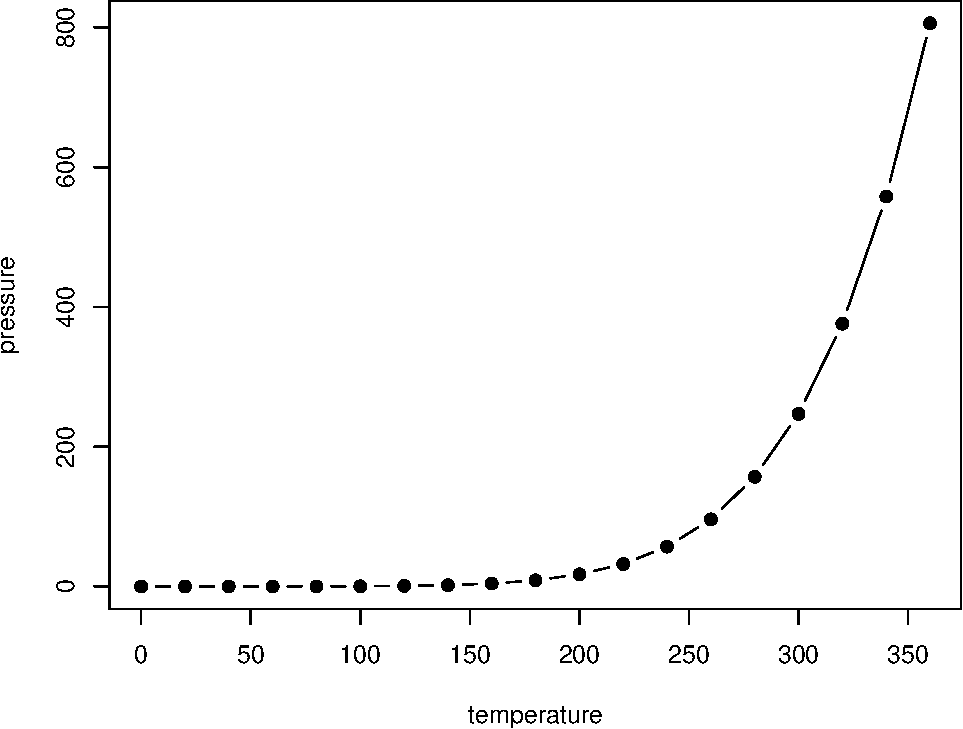
\includegraphics[width=0.8\linewidth]{_main_files/figure-latex/nice-fig-1} 

}

\caption{Here is a nice figure!}\label{fig:nice-fig}
\end{figure}

Don't miss Table \ref{tab:nice-tab}.

\begin{Shaded}
\begin{Highlighting}[]
\NormalTok{knitr}\SpecialCharTok{::}\FunctionTok{kable}\NormalTok{(}
  \FunctionTok{head}\NormalTok{(pressure, }\DecValTok{10}\NormalTok{), }\AttributeTok{caption =} \StringTok{\textquotesingle{}Here is a nice table!\textquotesingle{}}\NormalTok{,}
  \AttributeTok{booktabs =} \ConstantTok{TRUE}
\NormalTok{)}
\end{Highlighting}
\end{Shaded}

\begin{table}

\caption{\label{tab:nice-tab}Here is a nice table!}
\centering
\begin{tabular}[t]{rr}
\toprule
temperature & pressure\\
\midrule
0 & 0.0002\\
20 & 0.0012\\
40 & 0.0060\\
60 & 0.0300\\
80 & 0.0900\\
\addlinespace
100 & 0.2700\\
120 & 0.7500\\
140 & 1.8500\\
160 & 4.2000\\
180 & 8.8000\\
\bottomrule
\end{tabular}
\end{table}

\chapter{Parts}\label{parts}

You can add parts to organize one or more book chapters together. Parts can be inserted at the top of an .Rmd file, before the first-level chapter heading in that same file.

Add a numbered part: \texttt{\#\ (PART)\ Act\ one\ \{-\}} (followed by \texttt{\#\ A\ chapter})

Add an unnumbered part: \texttt{\#\ (PART\textbackslash{}*)\ Act\ one\ \{-\}} (followed by \texttt{\#\ A\ chapter})

Add an appendix as a special kind of un-numbered part: \texttt{\#\ (APPENDIX)\ Other\ stuff\ \{-\}} (followed by \texttt{\#\ A\ chapter}). Chapters in an appendix are prepended with letters instead of numbers.

\chapter{Footnotes and citations}\label{footnotes-and-citations}

\section{Footnotes}\label{footnotes}

Footnotes are put inside the square brackets after a caret \texttt{\^{}{[}{]}}. Like this one \footnote{This is a footnote.}.

\section{Citations}\label{citations}

Reference items in your bibliography file(s) using \texttt{@key}.

For example, we are using the \textbf{bookdown} package \citep{R-bookdown} (check out the last code chunk in index.Rmd to see how this citation key was added) in this sample book, which was built on top of R Markdown and \textbf{knitr} \citep{xie2015} (this citation was added manually in an external file book.bib).
Note that the \texttt{.bib} files need to be listed in the index.Rmd with the YAML \texttt{bibliography} key.

The RStudio Visual Markdown Editor can also make it easier to insert citations: \url{https://rstudio.github.io/visual-markdown-editing/\#/citations}

\chapter{Blocks}\label{blocks}

\section{Equations}\label{equations}

Here is an equation.

\begin{equation} 
  f\left(k\right) = \binom{n}{k} p^k\left(1-p\right)^{n-k}
  \label{eq:binom}
\end{equation}

You may refer to using \texttt{\textbackslash{}@ref(eq:binom)}, like see Equation \eqref{eq:binom}.

\section{Theorems and proofs}\label{theorems-and-proofs}

Labeled theorems can be referenced in text using \texttt{\textbackslash{}@ref(thm:tri)}, for example, check out this smart theorem \ref{thm:tri}.

\begin{theorem}
\protect\hypertarget{thm:tri}{}\label{thm:tri}For a right triangle, if \(c\) denotes the \emph{length} of the hypotenuse
and \(a\) and \(b\) denote the lengths of the \textbf{other} two sides, we have
\[a^2 + b^2 = c^2\]
\end{theorem}

Read more here \url{https://bookdown.org/yihui/bookdown/markdown-extensions-by-bookdown.html}.

\section{Callout blocks}\label{callout-blocks}

The R Markdown Cookbook provides more help on how to use custom blocks to design your own callouts: \url{https://bookdown.org/yihui/rmarkdown-cookbook/custom-blocks.html}

\chapter{Sharing your book}\label{sharing-your-book}

\section{Publishing}\label{publishing}

HTML books can be published online, see: \url{https://bookdown.org/yihui/bookdown/publishing.html}

\section{404 pages}\label{pages}

By default, users will be directed to a 404 page if they try to access a webpage that cannot be found. If you'd like to customize your 404 page instead of using the default, you may add either a \texttt{\_404.Rmd} or \texttt{\_404.md} file to your project root and use code and/or Markdown syntax.

\section{Metadata for sharing}\label{metadata-for-sharing}

Bookdown HTML books will provide HTML metadata for social sharing on platforms like Twitter, Facebook, and LinkedIn, using information you provide in the \texttt{index.Rmd} YAML. To setup, set the \texttt{url} for your book and the path to your \texttt{cover-image} file. Your book's \texttt{title} and \texttt{description} are also used.

This \texttt{gitbook} uses the same social sharing data across all chapters in your book- all links shared will look the same.

Specify your book's source repository on GitHub using the \texttt{edit} key under the configuration options in the \texttt{\_output.yml} file, which allows users to suggest an edit by linking to a chapter's source file.

Read more about the features of this output format here:

\url{https://pkgs.rstudio.com/bookdown/reference/gitbook.html}

Or use:

\begin{Shaded}
\begin{Highlighting}[]
\NormalTok{?bookdown}\SpecialCharTok{::}\NormalTok{gitbook}
\end{Highlighting}
\end{Shaded}


  \bibliography{book.bib,packages.bib}

\end{document}
